% Fable proposal (latex_review/fable/proposed). Generated by gen_fable_snippets.py; do not hand-edit values.
% Source: fable/exhibits/house_stock_grid.png sha256 41009c619d54faa3e598808ae121defe09b82d34806dcfd3aaec1bbe7a38d7e5
\begin{figure}[p]
\centering
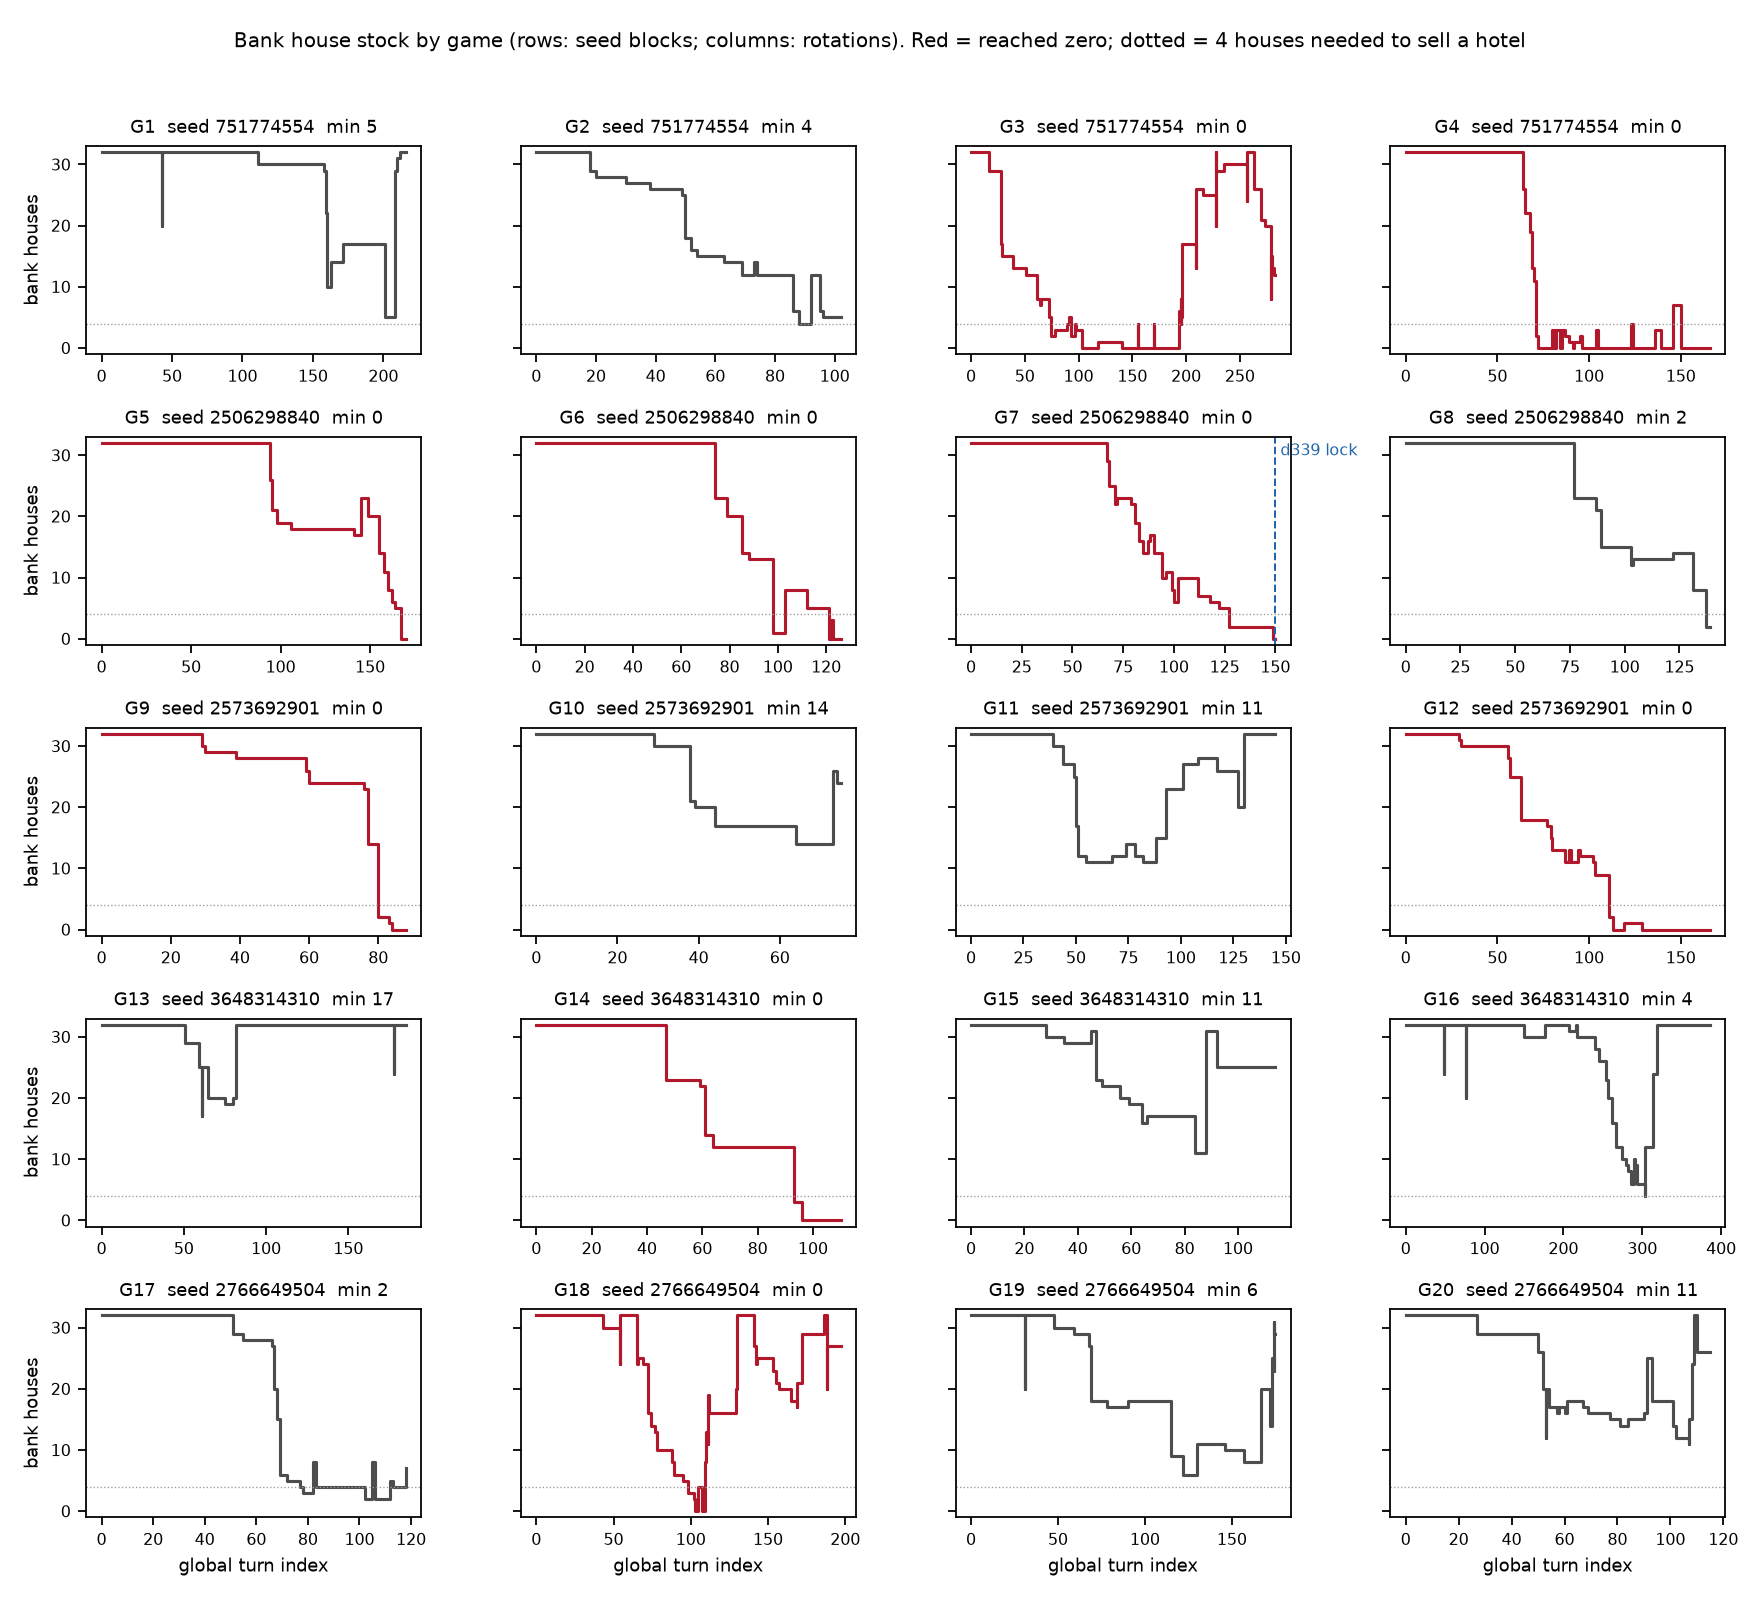
\includegraphics[width=\linewidth,height=0.8\textheight,keepaspectratio]{house_stock_grid.png}
\caption[Bank house stock by game (Fable)]{Bank houses remaining after each building event, by seed block (rows) and rotation (columns). Red marks games that reach zero; the dotted line is the four-house threshold needed to sell a hotel; the G7 d339 lock is marked. Hotel conversions return houses and produce upward steps. This is inventory and exposure, not a count of blocked builds or of demand. Raster include (PNG, 1760$\times$1600 px at 160 dpi; about 270 dpi effective at a 6.5 in width); regenerable as vector by \path{fable/scripts/house_stock_series.py}. Underlying data: Table~\ref{tab:fable_stock} and \path{fable/exhibits/house_stock_series.csv}.}
\label{fig:fable_stock_grid}
\end{figure}
